\begin{frame}
	\frametitle{Monop\'olio}
	\begin{itemize}
		\setlength\itemsep{1.2em}
		\item<1-> Uma s\'o empresa produz um bem sem substitutos pr\'oximos
		\item<2-> H\'a barreiras \`a entrada no mercado:\onslide<3->{\footnote{\onslide<3->{1 e 2 s\~ao barreiras legais; 3 e 4 s\~ao barreiras estruturais ou naturais.}}}
		\begin{enumerate}
			\setlength\itemsep{1.1em}
			\item<3-> Acesso exclusivo a inputs/licen\c cas de explora\c c\~ao
			\item<3-> Patentes, regulamenta\c c\~oes
			\item<3-> Custos de entrada muito elevados
			\item<3-> Tecnologia com rendimentos crescentes \`a escala/economias de escala
		\end{enumerate}
	\end{itemize}
\end{frame}

\begin{frame}
	\frametitle{Maximiza\c c\~ao de lucro}
	A empresa pretende encontrar a quantidade a produzir tal que:\[\max\ \Pi = RT-CT\]
	\begin{columns}
		\begin{column}{0.47\textwidth}
			\begin{center}
				{\color{blue}Concorr\^encia perfeita}\par
				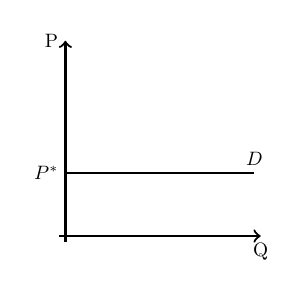
\begin{tikzpicture}[
					scale = 0.8,
					every node/.style = {scale = 0.7}
					]
					\draw[->,thick] (-0.1,0) -- (3.1,0)node[below]{Q};
					\draw[->,thick] (0,-0.1) -- (0,3.1)node[left]{P};

					\draw[thick] (0,1)node[left]{$P^*$} -- (3,1)node[above]{$D$};

				\end{tikzpicture}
				\[RT=P\times Q\]
			\end{center}
		\end{column}
		\begin{column}{0.47\textwidth}
			\begin{center}
				{\color{blue}Monop\'olio}\par
				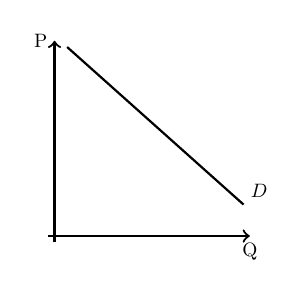
\begin{tikzpicture}[
					scale = 0.8,
					every node/.style = {scale = 0.7}
					]
					\draw[->,thick] (-0.1,0) -- (3.1,0)node[below]{Q};
					\draw[->,thick] (0,-0.1) -- (0,3.1)node[left]{P};

					\draw[thick] (0.2,3) -- (3,0.5)node[above right]{$D$};

				\end{tikzpicture}
				\[RT=P(Q)\times Q\]
			\end{center}
		\end{column}
	\end{columns}
\end{frame}

\begin{frame}
	\frametitle{Maximiza\c c\~ao do Lucro}
		Sendo \[\Pi = p(Q)\times Q - CV(Q) - CF\] 

		\pause

		A condi\c c\~ao de primeiro ordem (CPO) ser\'a: \pause
		\begin{align*}
			\frac{d\Pi}{dQ}=0 \Leftrightarrow \underbrace{p(Q)+Q\frac{dP(Q)}{dQ}}_{Rmg} - CV' = 0 \Leftrightarrow Rmg = Cmg > 0\
		\end{align*}\pause



		E a condi\c c\~ao de segundo ordem (CSO) ser\'a: \pause
		\begin{align*}
			\frac{d^2\Pi}{dQ^2} < 0 \Leftrightarrow \frac{dRmg}{dQ} < \frac{dCmg}{dQ}
		\end{align*}
\end{frame}

\begin{frame}
	\frametitle{Receita Marginal e Elasticidade da Procura}
	\begin{align*}
		\onslide<1->{Rmg &= Cmg > 0}\\
		\onslide<2->{Rmg &=P+Q\frac{dP}{dQ}}\\
		\onslide<3->{Rmg &=p\left(1+\frac{Q}{P}\frac{dP}{dQ}\right)}\\
		\onslide<4->{Rmg &=p\left(1+\frac{1}{\frac{P}{Q}\frac{dQ}{dP}}\right)}\\
		\onslide<5->{Rmg &= p\left(1+\frac{1}{\varepsilon_D}\right) = p \left(1-\frac{1}{|\varepsilon_D|}\right)}
	\end{align*}

\end{frame}

\begin{frame}
	\frametitle{Receita Marginal e Elasticidade da Procura}
	\begin{itemize}
		\item<1-> Sendo $\varepsilon_D=\frac{dQ}{dP}\frac{P}{Q}$ a elasticidade pre\c co da procura.
		\item<2-> A receita marginal s\'o ser\'a positiva na zona el\'astica da procura! Ent\~ao: 
		\item<3-> Se a procura \'e r\'igida, a $Rmg$ \'e negativa: se aumentar $Q$ colocada no mercado (por via de redu\c c\~ao de pre\c co), a Receita diminui (efeito pre\c co sobrep\~oe-se ao efeito quantidade), pelo que o monopolista nunca actuar\'a na zona r\'igida da procura...
	\end{itemize}

\end{frame}

\begin{frame}
	\frametitle{Receita Marginal e elasticidade}
	\begin{itemize}
		\setlength{\itemsep}{1.2em}
		\item<1-> NB: a receita do monopolista \'e igual \`a despesa de consumo...
		\item<2-> Revisitando o cap\'itulo 3A: qual a rela\c c\~ao entre altera\c c\~ao de pre\c co, despesa de consumo e elasticidade?
		\item<3-> Qual a implica\c c\~ao, sobre a despesa de consumo, do facto de o monopolista actuar apenas na zona el\'astica da procura?
	\end{itemize}
\end{frame}


\begin{frame}
	\frametitle{Elasticidade e Despesa de Consumo}
	\begin{columns}
		\begin{column}{0.47\textwidth}
			Generalizando os Resultados:
			\begin{align*}
				Despesa&=RT=P\times Q\\
				P&=\frac{a}{b}-\frac{1}{b}Q\\
				RT&=\left(\frac{a}{b}-\frac{1}{b}Q\right)\times Q\\
				&=\frac{a}{b}Q-\frac{1}{b}Q^2\\
				Rmg&=RT'=\frac{a}{b}-\frac{2}{b}Q\\
				Rmg&=0\Leftrightarrow Q=\frac{a}{2}
			\end{align*}
		\end{column}
		\begin{column}{0.47\textwidth}
			\begin{center}
				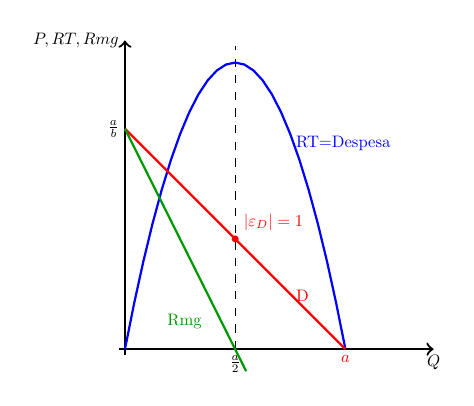
\begin{tikzpicture}[
					scale = 0.7,
					every node/.style = {scale = 0.6},
					declare function = {
						d(\x)=4-\x;
						rt(\x) = 1.3*(4-(\x-2)^2);
						rm(\x) = 4-(2)*\x;
					}]

					\draw[->,thick] (-0.1,0) -- (5.6,0)node[below]{$Q$};
					\draw[->,thick] (0,-0.1) -- (0,5.6)node[left]{$P,RT,Rmg$};
				
					\draw[dashed] (2,0)node[below]{$\frac{a}{2}$} -- (2,5.5);

					\draw[blue,thick,domain=0:4,variable=\x] plot (\x,{rt(\x)});
					\draw[blue] (3,3.5)node[above right]{RT=Despesa};

					\draw[red,thick,domain=0:4,variable=\x] plot (\x,{d(\x)}) node[below]{$a$};
					\draw[red] (3,0.75)node[above right]{D};	
					\draw[red] (2,2)node[circle,fill,inner sep=1.5,label=above right:{\(|\varepsilon_D|=1\)}]{};

					\draw[green!60!black,thick,domain=0:2.2,variable=\x] plot (\x,{rm(\x)});
					\draw[green!60!black] (1.5,0.5)node[left]{Rmg};
					\draw(0,{rm(0)}) node[left]{$\frac{a}{b}$};

				\end{tikzpicture}
			\end{center}
		\end{column}
	\end{columns}
\end{frame}

\begin{frame}
	\frametitle{Monop\'olio com procura linear}
	\begin{columns}
		\begin{column}{0.47\textwidth}
			\begin{center}
				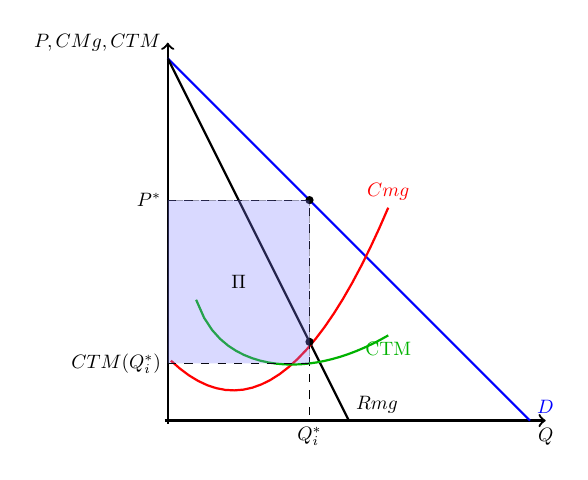
\begin{tikzpicture}[
					scale = 0.4,
					every node/.style = {scale =0.7},
					declare function = {
						d(\x) = 11.5-\x;
						rt(\x) = \x*d(\x);
						rmg(\x) = d(\x) - \x;
						cv(\x) = \x - (1/4)*\x^2 + (1/25)*\x^3;
						cf(\x) = 1;
						ct(\x) = cv(\x) + cf(\x);
						cmg(\x) = 1 - (2/4)*\x + (3/25)*\x^2;
						ctm(\x) = ct(\x)/\x;
					}
				]
					\def\p{4.5}

					\draw[->,thick] (-0.1,-0) -- (12,-0) node[below]{$Q$};
					\draw[->,thick] (0,-0.1) -- (0,12) node[left]{$P,CMg,CTM$};

					\onslide<1->{
						\draw[blue,thick,domain=0:11.5,variable=\x] plot (\x,{d(\x)})node[above right]{$D$};
						\draw[thick,domain=0:5.75,variable=\x] plot (\x,{rmg(\x)})node[above right]{$Rmg$};
					}

					\onslide<2->{
						\draw[red,thick,domain=0.1:7,variable=\x] plot (\x,{2*cmg(\x)-0})node[above]{$Cmg$};
					}

					\onslide<3->{
						\draw (\p,{rmg(\p)}) node[circle,fill,inner sep=1.5]{};
					}

					\onslide<4->{
						\draw[dashed] (0,{d(\p)})node[left]{$P^*$} -- (\p,{d(\p)})node[circle,fill,inner sep=1.5]{} -- (\p,0)node[below]{$Q_i^*$};		
					}

					\onslide<5->{
						\draw[green!70!black,thick,domain=0.9:7,variable=\x] plot (\x,{2*ctm(\x)-0})node[below]{CTM};
					}

					\onslide<6->{
						\draw[dashed] (0,{2*ctm(\p)})node[left]{$CTM(Q_i^*)$} -- (\p,{2*ctm(\p)});		
					}

					\onslide<7->{
						\draw[dashed,fill=blue!50!white,opacity=0.3] (0,{2*ctm(\p)}) -- (\p,{2*ctm(\p)}) --(\p,{d(\p)}) -- (0,{d(\p)}) -- (0,{2*ctm(\p)});
						\draw({\p/2},{(d(\p)+2*ctm(\p))/2}) node{$\Pi$};
					}	

				\end{tikzpicture}
			\end{center}
		\end{column}
		\begin{column}{0.47\textwidth}
			\begin{center}
				\onslide<2->{\(P=a-bQ\)}
				\onslide<3->{\(\Rightarrow RT=aQ-bQ^2\)}
				\onslide<4->{\(Rmg=RT'=a-2bQ\)}
				\vspace{0.25cm}
				\onslide<5->{
					\par \justify A curva da receita marginal tem o dobro do declive (em m\'odulo) da curva inversa da procura.\par
				}
				\onslide<7->{
					\[\Pi = RT-CT=Q(P-CTM)\]
				}

			\end{center}
		\end{column}
	\end{columns}
\end{frame}

\begin{frame}
	\frametitle{Excedente Econ\'omico em monop\'olio}
	\begin{center}
		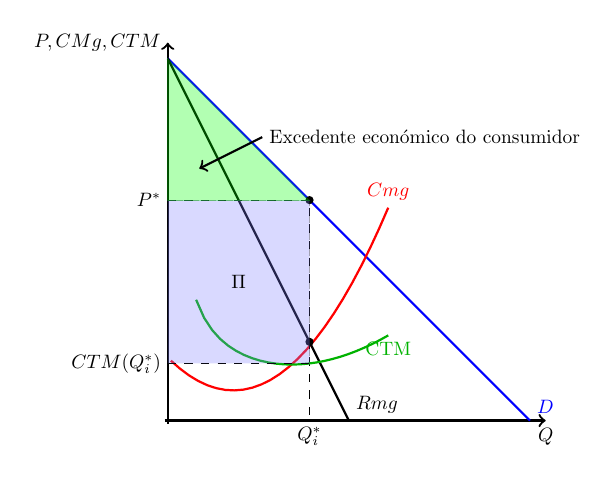
\begin{tikzpicture}[
			scale = 0.4,
			every node/.style = {scale =0.7},
			declare function = {
				d(\x) = 11.5-\x;
				rt(\x) = \x*d(\x);
				rmg(\x) = d(\x) - \x;
				cv(\x) = \x - (1/4)*\x^2 + (1/25)*\x^3;
				cf(\x) = 1;
				ct(\x) = cv(\x) + cf(\x);
				cmg(\x) = 1 - (2/4)*\x + (3/25)*\x^2;
				ctm(\x) = ct(\x)/\x;
			}
			]
			\def\p{4.5}

			\draw[->,thick] (-0.1,-0) -- (12,-0) node[below]{$Q$};
			\draw[->,thick] (0,-0.1) -- (0,12) node[left]{$P,CMg,CTM$};

			\draw[blue,thick,domain=0:11.5,variable=\x] plot (\x,{d(\x)})node[above right]{$D$};

			\draw[red,thick,domain=0.1:7,variable=\x] plot (\x,{2*cmg(\x)-0})node[above]{$Cmg$};
			\draw[thick,domain=0:5.75,variable=\x] plot (\x,{rmg(\x)})node[above right]{$Rmg$};

			\draw (\p,{rmg(\p)}) node[circle,fill,inner sep=1.5]{};

			\draw[dashed] (0,{d(\p)})node[left]{$P^*$} -- (\p,{d(\p)})node[circle,fill,inner sep=1.5]{} -- (\p,0)node[below]{$Q_i^*$};		

			\draw[green!70!black,thick,domain=0.9:7,variable=\x] plot (\x,{2*ctm(\x)-0})node[below]{CTM};

			\draw[dashed] (0,{2*ctm(\p)})node[left]{$CTM(Q_i^*)$} -- (\p,{2*ctm(\p)});		

			\draw[dashed,fill=blue!50!white,opacity=0.3] (0,{2*ctm(\p)}) -- (\p,{2*ctm(\p)}) --(\p,{d(\p)}) -- (0,{d(\p)}) -- (0,{2*ctm(\p)});
			\draw({\p/2},{(d(\p)+2*ctm(\p))/2}) node{$\Pi$};

			\draw[fill,green,opacity=0.3] (0,{d(0)}) -- (0,{d(\p)}) -- (\p,{d(\p)});

			\draw[thick,->] (3,9)node[right]{Excedente econ\'omico do consumidor} -- (1,8);

		\end{tikzpicture}
		\onslide<2->{\par E o excedente econ\'omico do produtor?}
	\end{center}	
\end{frame}

\begin{frame}
	\frametitle{Oferta em monop\'olio?}
	\begin{columns}
		\begin{column}{0.47\textwidth}
			\onslide<1->{
				Em concorr\^encia perfeita
				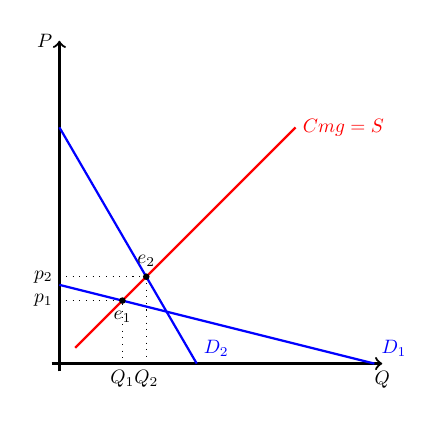
\begin{tikzpicture}[
						every node/.style = {scale = 0.7},
						declare function = {
							d1(\x) = 1-0.25*\x;
							d2(\x) = 3-1.72*\x;
							cmg(\x) = \x;
						}]

					\def\eqa{4/5}
					\def\eqb{3/2.72}

					\draw[thick,->](-0.1,0) --  (4.1,0)node[below]{$Q$};
					\draw[thick,->](0,-0.1) --  (0,4.1)node[left]{$P$};

					\draw[blue,thick,domain=0:4,variable=\x] plot (\x,{d1(\x)})node[above right]{$D_1$};
					\draw[blue,thick,domain=0:1.744,variable=\x] plot (\x,{d2(\x)})node[above right]{$D_2$};
					\draw[red,thick,domain=0.2:3,variable=\x] plot (\x,{cmg(\x)})node[right]{$Cmg=S$};

					\draw[dotted] (0,{cmg(\eqa)})node[left]{$p_1$} -- (\eqa,{cmg(\eqa)})node[circle,fill,inner sep=1.2,label=below:{$e_1$}]{} -- (\eqa,0)node[below]{$Q_1$};
					\draw[dotted] (0,{cmg(\eqb)})node[left]{$p_2$} -- (\eqb,{cmg(\eqb)})node[circle,fill,inner sep=1.2,label=above:{$e_2$}]{} -- (\eqb,0)node[below]{$Q_2$};

				\end{tikzpicture}
			}
		\end{column}
		\begin{column}{0.47\textwidth}
			\onslide<2->{
				Em monop\'olio
				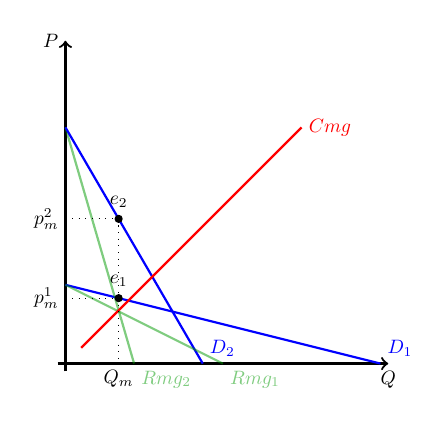
\begin{tikzpicture}[
						every node/.style = {scale = 0.7},
						declare function = {
							d1(\x) = 1-0.25*\x;
							rmg1(\x) = d1(\x) - 0.25*\x;							
							d2(\x) = 3-1.72*\x;
							rmg2(\x) = d2(\x) - 1.72*\x;
							cmg(\x) = \x;
						}]
	
					\def\eq{3/4.44}

					\draw[thick,->](-0.1,0) --  (4.1,0)node[below]{$Q$};
					\draw[thick,->](0,-0.1) --  (0,4.1)node[left]{$P$};

					\draw[blue,thick,domain=0:4,variable=\x] plot (\x,{d1(\x)})node[above right]{$D_1$};
					\draw[green!60!black,opacity=0.5,thick,domain=0:0.872,variable=\x] plot (\x,{rmg2(\x)})node[below right]{$Rmg_2$};

					\draw[blue,thick,domain=0:1.744,variable=\x] plot (\x,{d2(\x)})node[above right]{$D_2$};
					\draw[green!60!black,opacity=0.5,thick,domain=0:2,variable=\x] plot (\x,{rmg1(\x)})node[below right]{$Rmg_1$};
					
					\draw[red,thick,domain=0.2:3,variable=\x] plot (\x,{cmg(\x)})node[right]{$Cmg$};

					\draw[dotted] (0,{d1(\eq)})node[left]{$p_m^1$} -- (\eq,{d1(\eq)})node[circle,fill,inner sep=1.5,label=above:{$e_1$}]{} -- (\eq,0)node[below]{$Q_m$};

					\draw[dotted] (0,{d2(\eq)})node[left]{$p_m^2$} -- (\eq,{d2(\eq)})node[circle,fill,inner sep=1.5,label=above:{$e_2$}]{} -- (\eq,{d1(\eq)});

				\end{tikzpicture}
			}
		\end{column}
	\end{columns}
	\onslide<3->{
		\par No caso do monop\'olio \emph{\underline{podemos}} ter a mesma quantidade,\footnote{\onslide<3->{Poder n\~ao quer dizer que \'e um resultado garantido, s\'o poss\'ivel.}} e dois pre\c cos para duas procuras distintas!\par Assim ent\~ao, n\~ao podemos ter uma fun\c c\~ao oferta.
	}
\end{frame}

\begin{frame}
	\frametitle{Oferta em monop\'olio?}
	A rela\c c\~ao pre\c co quantidade depende da procura!, pelo que n\~ao existe uma oferta como a conhecemos.\par

	\vspace{1em}

	Assim, termos que calcular o excedente do produtor como vimos na defini\c c\~ao original, ou seja, como a receita menos os custos vari\'aveis.
\end{frame}

\begin{frame}
	\frametitle{Monopolista n\~ao produz}
	\begin{center}
		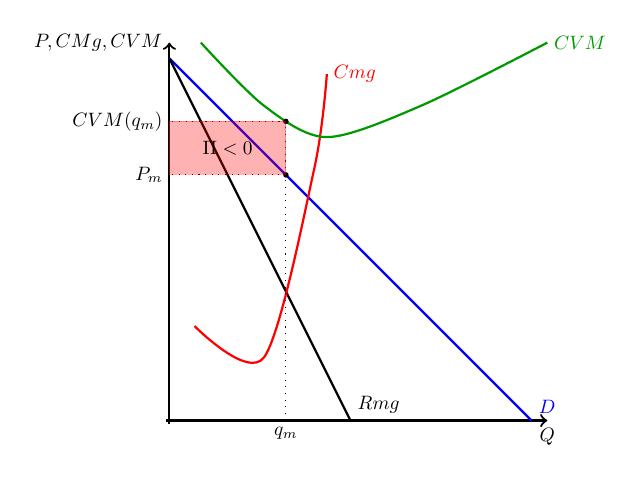
\begin{tikzpicture}[
			scale = 0.4,
			every node/.style = {scale =0.7},
			declare function = {
				d(\x) = 11.5-\x;
				rt(\x) = \x*d(\x);
				rmg(\x) = d(\x) - \x;
				cv(\x) = 4*(\x-4)- (1/4)*(\x-4)^2 + (1/25)*(\x-4)^3;
				cf(\x) = 1;
				ct(\x) = cv(\x) + cf(\x);
				cmg(\x) = 4 - (2/4)*(\x-4) + (3/25)*(\x-4)^2;
				ctm(\x) = ct(\x)/\x;
				cvm(\x) = cv(\x)/(\x-4);
			}
			]
			\def\p{4.5}

			\draw[->,thick] (-0.1,-0) -- (12,-0) node[below]{$Q$};
			\draw[->,thick] (0,-0.1) -- (0,12) node[left]{$P,CMg,CVM$};

			\draw[blue,thick,domain=0:11.5,variable=\x] plot (\x,{d(\x)})node[above right]{$D$};

			\draw[thick,domain=0:5.75,variable=\x] plot (\x,{rmg(\x)})node[above right]{$Rmg$};

			\draw[smooth,red,thick] plot coordinates {(0.8,3) (3,2) (4.6,8) (5,11)};
			\draw[smooth,green!60!black,thick] plot coordinates {(1,12) (3,10) (5,9) (8,10) (12,12)};

			\draw[red](5,11)node[right]{$Cmg$};
			\draw[green!60!black](12,12)node[right]{$CVM$};

			\def\qa{3.7}
			\def\vca{9.5}

			\onslide<2->{
				\draw[dotted] (\qa,0)node[below]{$q_m$} -- (\qa,\vca)node[circle,fill,inner sep=1]{} -- (0,\vca)node[left]{$CVM(q_m)$};
				\draw[dotted] (\qa,{d(\qa)})node[circle,fill,inner sep=1]{} -- (0,{d(\qa)})node[left]{$P_m$};
			}

			\onslide<3->{
				\draw[fill,red,opacity=0.3] (0,{d(\qa)}) -- (0,\vca) -- (\qa,\vca) -- (\qa,{d(\qa)});
				\draw[black] ({\qa/2},{(d(\qa)+\vca)/2}) node[black]{$\Pi<0$};
			}
		\end{tikzpicture}

		\onslide<4->{
			\par A procura seria demasiado pequena para os custos da ind\'ustria
		}

	\end{center}	
\end{frame}

\begin{frame}
	\frametitle{Monop\'olio vs. Concorr\^encia Perfeita}
	\begin{center}
		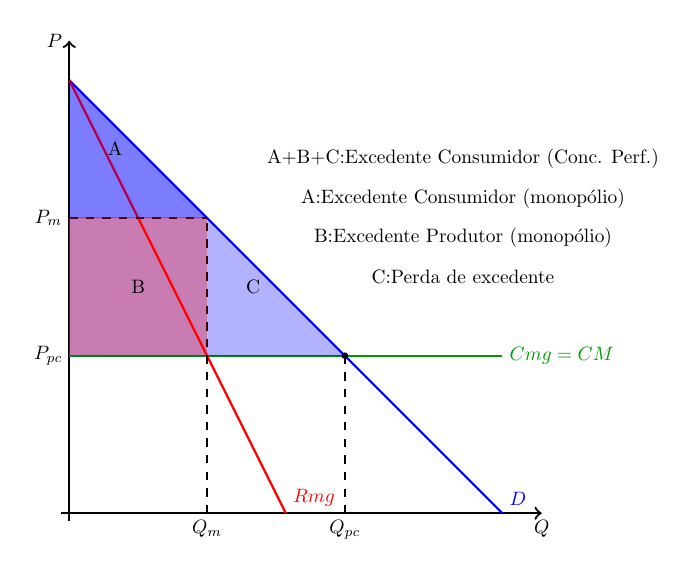
\begin{tikzpicture}[
			scale = 1,
			every node/.style = {scale =0.7},
			declare function = {
				d(\x) = 5.5-\x;
				rmg(\x) = 5.5-2*\x;
				cmg(\x) = 2;
			}
			]

			\def\eqcp{3.5}
			\def\eqcm{3.5/2}

			\draw[->,thick] (-0.1,-0) -- (6,-0) node[below]{$Q$};
			\draw[->,thick] (0,-0.1) -- (0,6) node[left]{$P$};

			\draw[thick,blue,domain=0:5.5,variable=\x] plot (\x,{d(\x)}) node[above right]{$D$};
			\draw[thick,green!60!black,domain=0:5.5,variable=\x] plot (\x,{cmg(\x)}) node[right]{$Cmg=CM$}; 

			\onslide<2->{
				\draw (0,{cmg(0)}) node[left]{$P_{pc}$};
				\draw[dashed,thick] (\eqcp,{d(\eqcp)})node[circle,fill,inner sep=1.2]{} -- (\eqcp,0) node[below]{$Q_{pc}$};
			}

			\onslide<3-6>{
				\draw[fill,blue,opacity=0.3] (0,{d(0)}) -- (\eqcp,{d(\eqcp)}) -- (0,{d(\eqcp)});
			}

			\onslide<4->{
				\draw[thick,red,domain=0:2.75,variable=\x] plot (\x,{rmg(\x)}) node[above right]{$Rmg$};
			}

			\onslide<5->{
				\draw[dashed,thick] (\eqcm,0)node[below]{$Q_m$} -- (\eqcm,{d(\eqcm)});
			}

			\onslide<6->{
				\draw[dashed,thick] (0,{d(\eqcm)})node[left]{$P_m$} -- (\eqcm,{d(\eqcm)});
			}

			\onslide<7->{
				\draw[fill,blue,opacity=0.3] (0,{d(0)}) -- (\eqcm,{d(\eqcm)}) -- (0,{d(\eqcm)});
				\draw[fill,red,opacity=0.3] (\eqcm,{d(\eqcm)}) -- (0,{d(\eqcm)}) -- (0,{d(\eqcp)}) -- (\eqcm,{d(\eqcp)});
			}

			\onslide<8->{
				\draw({\eqcm/3},{(d(\eqcm)+d(0))/2})node[]{A};
				\draw({\eqcm/2},{(d(\eqcm)+d(\eqcp))/2})node[]{B};
				\draw({\eqcm+(\eqcp-\eqcm)/3},{(d(\eqcm)+d(\eqcp))/2})node[]{C};
			}

			\onslide<9->{
				\draw(5,4.5) node[]{A+B+C:Excedente Consumidor (Conc. Perf.)};
				\draw(5,4) node[]{A:Excedente Consumidor (monop\'olio)};
				\draw(5,3.5) node[]{B:Excedente Produtor (monop\'olio)};
				\draw(5,3) node[]{C:Perda de excedente};
			}

		\end{tikzpicture}
	\end{center}
\end{frame}

\begin{frame}
	\frametitle{Nem sempre \'e vi\'avel um mercado concorrencial...}
	\begin{columns}
		\begin{column}{0.3\textwidth}
			\onslide<8->{\footnotesize
				\textbf{Economias de Escala:}
				limitam o n\'umero de empresas no mercado, constituindo ``barreiras naturais'' \`a entrada de empresas, dando \underline{poder de mercado} \`as empresas instaladas.. no limite, pode haver uma s\'o...
			}
		\end{column}
		\begin{column}{0.7\textwidth}
			\begin{center}
				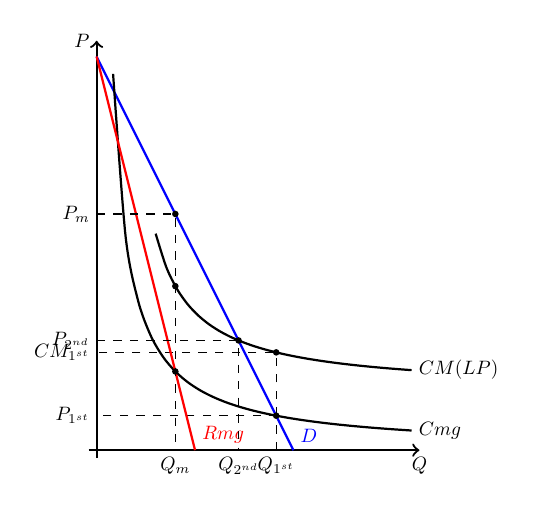
\begin{tikzpicture}[
					scale = 1,
					every node/.style = {scale =0.7},
					declare function = {
						d(\x) = 5-2*\x;
						rmg(\x) = 5-4*\x;
						cmg(\x) = 1/\x;
						cm(\x) = 1/(\x-0.25)+0.75;
					}
					]

					\def\qaa{2.2808} %1st best
					\def\qab{0.21922} % 1st worst
					\def\qba{1} % monop
					\def\qbb{1/4} %monop corte esq
					\def\qca{1.8031} % q of CMLP = D
					\def\qcb{0.57195} %
					

					\draw[->,thick] (-0.1,-0) -- (4.1,-0) node[below]{$Q$};
					\draw[->,thick] (0,-0.1) -- (0,5.2) node[left]{$P$};

					\onslide<2->{
						\draw[thick,blue,domain=0:2.5,variable=\x] plot (\x,{d(\x)}) node[above right]{$D$};
						\draw[thick,domain=(\qab-0.01):4,variable=\x,smooth] plot (\x,{cmg(\x)}) node[right]{$Cmg$};
					}

					\onslide<3-9>{
						\draw[dashed] (\qaa,0)node[below]{$Q_{1^{st}}$} -- (\qaa,{d(\qaa)}) node[circle,fill,inner sep=1.2]{} -- (0,{d(\qaa)}) node[left]{$P_{1^{st}}$};
					}

					\onslide<4->{
						\draw[thick,domain=0.75:4,variable=\x,smooth] plot (\x,{cm(\x)}) node[right]{$CM(LP)$};					
					}

					\onslide<5-9>{
						\draw[dashed] (\qaa,{d(\qaa)}) -- (\qaa,{cm(\qaa)})node[circle,fill,inner sep=1.2]{} -- (0,{cm(\qaa)})node[left]{$CM_{1^{st}}$};
					}

					\onslide<6->{
						\draw[thick,red,domain=0:1.25,variable=\x] plot (\x,{rmg(\x)}) node[above right]{$Rmg$};
					}

					\onslide<7-9>{
						\draw[dashed] (0,{d(\qba)})node[left]{$P_m$} -- (\qba,{d(\qba)})node[circle,fill,inner sep=1.2]{} -- (\qba,{cm(\qba)})node[circle,fill,inner sep=1.2]{} -- (\qba,{cmg(\qba)})node[circle,fill,inner sep=1.2]{} -- (\qba,0)node[below]{$Q_m$};
					}

					\onslide<10->{
						\draw[dashed] (0,{d(\qca)})node[left]{$P_{2^{nd}}$} -- (\qca,{d(\qca)})node[circle,fill,inner sep=1.2]{} -- (\qca,0)node[below]{$Q_{2^{nd}}$};
					}

				\end{tikzpicture}
			\end{center}
		\end{column}
	\end{columns}
	\onslide<9>{\footnotesize 1\textsuperscript{st} best ($P=Cmg$) n\~ao \'e vi\'avel na presen\c ca de Economias de Escala, j\'a que \'e um pre\c co que iria gerar um preju\'izo permanente.\par}
	\onslide<10>{\footnotesize E se pud\'essemos optar por um 2\textsuperscript{nd} best ($P=CM(LP)$)}
\end{frame}